\documentclass[11pt,a4paper]{article}
\usepackage[a4paper,top=20mm,bottom=19mm,left=19mm,right=19mm]{geometry}
\usepackage{fontspec}
\setmainfont{TeX Gyre Pagella}
\setsansfont{TeX Gyre Heros}
\setmonofont{Latin Modern Mono}
\usepackage{booktabs,tabularx,array,amsmath,amssymb}
\usepackage{xcolor,tcolorbox,graphicx,float,fancyhdr,hyperref,enumitem,microtype}
\usepackage{pgfplots}
\usepgfplotslibrary{groupplots}
\pgfplotsset{compat=1.18}
\definecolor{navy}{HTML}{17324D}
\definecolor{blue}{HTML}{3157D5}
\definecolor{orange}{HTML}{D56B2D}
\definecolor{ink}{HTML}{263442}
\definecolor{muted}{HTML}{66788A}
\definecolor{panel}{HTML}{F3F6FA}
\definecolor{rule}{HTML}{D8E0E8}
\hypersetup{colorlinks=true,linkcolor=navy,urlcolor=blue}
\setlength{\parindent}{0pt}
\setlength{\emergencystretch}{2em}
\setlength{\parskip}{0.5em}
\setlength{\headheight}{17pt}
\setlist{nosep,leftmargin=1.5em}
\renewcommand{\arraystretch}{1.18}
\pagestyle{fancy}
\fancyhf{}
\lhead{\small\textcolor{muted}{Sync2Act / Data Quality Study}}
\rhead{\small\textcolor{muted}{v1\_4\_0}}
\cfoot{\textcolor{muted}{\thepage}}
\renewcommand{\headrulewidth}{0.4pt}
\newcolumntype{Y}{>{\raggedright\arraybackslash}X}
\newcommand{\code}[1]{\texttt{\small #1}}
\newcommand{\note}[1]{\begin{tcolorbox}[colback=panel,colframe=rule,boxrule=0.5pt,arc=1mm]#1\end{tcolorbox}}
\newcommand{\metric}[1]{\textcolor{blue}{\bfseries #1}}

\usepackage{multirow,tocloft}
\setlength{\cftsecnumwidth}{2.8em}
\setlength{\cftbeforesecskip}{5pt}
\definecolor{teal}{HTML}{00A6A6}
\definecolor{purple}{HTML}{7456B8}
\definecolor{rose}{HTML}{D45576}
\definecolor{green}{HTML}{3B9A66}
\newcolumntype{C}[1]{>{\centering\arraybackslash}p{#1}}
\newcommand{\good}[1]{\textcolor{green}{\bfseries #1}}
\newcommand{\warn}[1]{\textcolor{orange}{\bfseries #1}}
\hypersetup{pdftitle={Sync2Act v1\_4\_0: Data Quality and Policy Robustness}}
\setcounter{tocdepth}{1}
\begin{document}
\thispagestyle{empty}
\vspace*{12mm}
{\color{blue}\rule{25mm}{2.5pt}}\\[7mm]
{\fontsize{30}{36}\selectfont\bfseries\color{navy}Sync2Act\par}
\vspace{5mm}
{\LARGE\bfseries\color{navy}Data Quality and Policy Robustness\par}
\vspace{4mm}{\large\color{muted}Learning from damaged demonstrations and predicting from damaged observations\par}
\vspace{5mm}{\large v1\_4\_0 / 2026-10-07}\par\vspace{6mm}
\note{How should known data-quality information enter an imitation-learning system? Using the same robot tasks and fixed models, this study connects damaged training demonstrations, corrupted test observations, and temporal ensembling of action chunks, separating learning-stage benefits from prediction-stage robustness.}
\begin{center}
\small
\begin{tabular}{lp{121mm}}
\toprule
Evidence & Scope \\
\midrule
Training and ablations & 3 datasets x 6 models x 5 conditions x 3 seeds = 270 \\
Test robustness & 4,158 evaluations, including 270 clean-baseline audits \\
Temporal ensembling & 270 paired runs; fixed decay=0.7 \\
\bottomrule
\end{tabular}
\end{center}
\textbf{Principal finding.} Correct action-label weighting mitigates damaged demonstrations: mean training-degradation ratios for Q-Full and ACT-Lite are 0.977 versus 2.432 under label damage, and 1.144 versus 1.535 under mixed damage. Yet with mixed-damage training, Q-Full has about 36.1\% higher paired MSE than ACT-Lite on ALOHA with medium state-corrupted tests, versus 3.0\% and 2.1\% lower on Koch and xArm. Learning-stage gains do not automatically confer robustness to damaged inputs.

Temporal ensembling at fixed decay=0.7 did not lower overall actual MSE: the mean per-run percentage change across 270 pairs was $+21.20\%$. Absolute errors and distinct paired ratios are reported together to avoid mistaking denominator changes for improved accuracy.

\vfill\note{This report integrates existing training and evaluation evidence without retraining. All results concern offline action prediction, not real-robot closed-loop success.}
\clearpage\begingroup\setlength{\parskip}{0pt}\tableofcontents\endgroup
\vspace{8mm}\note{Sections 1--4 define the shared experiment and metrics. Section 5 studies demonstration quality; Sections 6--7 examine test inputs and quality metadata. Section 8 evaluates action selection; Sections 9--10 give joint conclusions, limitations, and reproducibility. Appendices contain the complete corrupted-test matrices.}
\clearpage\section{Research questions and shared experimental design}
Data corruption can occur during learning or at model-use time. The former changes supervision and the learned policy; the latter changes the observations available for prediction. We test whether quality inputs and label weighting improve learning from damaged demonstrations, whether fixed models tolerate image/state faults, and whether temporal ensembling lowers error on the same trajectories.

\begin{center}
\small
\begin{tabular}{llp{94mm}}
\toprule
Training & Test & Role in this report \\
\midrule
Clean & Clean & Recomputed historical baseline \\
Damaged & Clean & Recomputed historical baseline \\
Clean & Damaged & New test-robustness results \\
Damaged & Damaged & New cross-condition results \\
\bottomrule
\end{tabular}
\end{center}\begin{center}
\footnotesize
\begin{tabular}{lrrrrrr}
\toprule
Dataset & Ep. & Frames & Cam. & S / A & Train / Val / Test & Test frames \\
\midrule
ALOHA & 49 & 29,400 & 4 & 14 / 14 & 41 / 4 / 4 & 2,400 \\
Koch & 100 & 32,951 & 2 & 6 / 6 & 80 / 10 / 10 & 3,342 \\
xArm & 800 & 20,000 & 1 & 4 / 4 & 640 / 80 / 80 & 2,000 \\
\bottomrule
\end{tabular}
\end{center}ALOHA is static-battery manipulation, Koch is single-Lego pick-and-place, and xArm is lifting; all passed the single-task check. Full episodes, frames, and synchronized cameras are used. Fixed episode partitions precede training corruption and separate corrupted test copies, preventing adjacent-frame leakage. Clean means no added synthetic faults, not proof that recordings are noise-free.

The split seed is 7; training seeds are 7, 17, and 27. Images have a 64-pixel maximum side; training uses 10 epochs, CUDA, batch size 256, and action horizon 8. Normalization is fitted once to clean training episodes per dataset and fixed across its 90 model/condition/seed combinations; tests restore it from checkpoints. Validation stays clean, and test faults never alter partitions or training statistics.

\clearpage\section{Model ablations and training corruption}
ACT-Lite is a lightweight action-chunk predictor that omits the original ACT CVAE path. Quality variants reuse its backbone and condition camera/state observations separately. BC-MLP is supported by the application but is not part of these 270 historical checkpoints.

\begin{center}
\small
\begin{tabular}{lp{68mm}l}
\toprule
Model & Training quality input & Label weighting \\
\midrule
ACT-Lite & None & No \\
Q-Input & True synthetic metadata & No \\
Q-Weighted & None & Yes \\
Q-Full & True synthetic metadata & Yes \\
Q-Shuffled & Shuffled quality metadata & Yes, shuffled values \\
Q-Constant & Constant normal metadata & Yes, constant values \\
\bottomrule
\end{tabular}
\end{center}
Training segments use the mixtures below; test observations use the separate recipes in the next section. C/I/S/A/M are training-condition abbreviations used in subsequent tables.

\begin{center}
\footnotesize
\begin{tabular}{lp{133mm}}
\toprule
Condition & Training segment composition \\
\midrule
C & 100\% clean \\
I & 50\% clean; 40\% image delay (2 frames); 10\% image missing \\
S & 50\% clean; 40\% state delay (2 frames); 10\% state missing \\
A & 50\% clean; 40\% action delay (2 frames); 10\% action-label missing \\
M & 20\% clean; 20\% each image/state delay; 25\% action delay; 5\% each image/state/action missing \\
\bottomrule
\end{tabular}
\end{center}
\note{All six variants receive the same true observation metadata in Oracle tests, including models trained with shuffled/constant metadata. Training ablations and inference-time metadata interventions are distinct controls. Action-label quality never weights test metrics.}
Q-Input, Q-Weighted, and Q-Full abbreviate Quality-Input, Quality-Weighted-Loss, and Quality-Full. Q-Shuffled breaks sample-quality correspondence; Q-Constant marks quality as normal. Missing images/state do not remove whole training samples. Missing actions concern label reliability; only label-quality-weighted loss reduces or removes their supervision contribution.

\clearpage\section{Fault injection and evaluation workflow}
\textbf{Training faults.} Contiguous 16-frame segments receive one exclusive mixture component, without double-counting. Training shifts use two frames with invalid boundaries marked missing; the affected input/label and quality are zeroed, with masks and provenance retained. Maximum segment-fraction deviation is about 0.03 percentage points; frame deviations reach about 0.35 for single-modality and 0.83 for mixed conditions because final segments can be shorter than 16 frames.

Test trajectories are divided into disjoint 16-frame segments with deterministic fault assignments. Delays read past observations within the same episode; missing inputs are zeroed. Unavailable boundary observations are marked missing. Frames are not removed, episodes are not crossed, and future frames are never read.

\[\widetilde{o}_t=o_{t-\Delta},\quad \Delta>0;\qquad \widetilde{a}^{\,\mathrm{target}}_t=a_t.\]
\begin{center}
\footnotesize
\begin{tabular}{lrrr}
\toprule
Severity & Delay frames & Single modality: delayed / missing & Mixed: delayed / missing \\
\midrule
Light & 1 & 0.20 / 0.05 & 0.30 / 0.10 \\
Medium & 2 & 0.40 / 0.10 & 0.60 / 0.20 \\
Heavy & 4 & 0.60 / 0.20 & 0.70 / 0.30 \\
\bottomrule
\end{tabular}
\end{center}
Single-modality conditions damage either images or state. Mixed conditions split the delayed and missing fractions equally between image and state. Medium mixed tests therefore use 20\% clean, 30\% image delay, 30\% state delay, 10\% image missing, and 10\% state missing. Remaining segments are clean.

Fractions allocate segments rather than independent frame-drop probabilities. Short final segments can shift actual affected-frame proportions; per-evaluation manifests record realized fractions and millisecond offsets. Test-damage seeds 107, 117, and 127 are separate from training seeds. Every model sees the same damaged inputs for a given dataset, condition, and damage seed.

\begin{center}
\small
\begin{tabular}{lcr}
\toprule
Evaluation group & Construction & Count \\
\midrule
Clean baseline & $270$ & 270 \\
Medium Oracle & $270\times3\times3$ & 2,430 \\
Unknown metadata & $90\times3\times3$ & 810 \\
Light / heavy & $36\times2\times3\times3$ & 648 \\
Total &  & \textbf{4,158} \\
\bottomrule
\end{tabular}
\end{center}
Unknown-metadata tests cover every training condition of Q-Input and Q-Full. Severity extensions cover ACT-Lite and Q-Full with C and M training. Light/medium/heavy jointly change delay and damaged fraction, so they are not single-factor sensitivity experiments.
\clearpage\section{Metrics, paired comparisons, and uncertainty}
Default evaluation takes the first action in each chunk and denormalizes it to original action units. MSE weights every test frame and action dimension equally; MAE is also computed. Quality never downweights test metrics, and action targets stay fixed. Raw MSE is not pooled across robots with different action scales.

\[E=\frac{1}{ND}\sum_{t=1}^{N}\sum_{j=1}^{D}(\hat a_{t,j}-a_{t,j})^2.\]
\begin{align*}
R_{\mathrm{train}}&=\frac{E_{\mathrm{damaged\ train,clean\ test}}}{E_{\mathrm{clean\ train,clean\ test}}},\\
R_{\mathrm{test}}&=\frac{E_{\mathrm{same\ checkpoint,damaged\ test}}}{E_{\mathrm{same\ checkpoint,clean\ test}}},\\
P&=\frac{E_{\mathrm{Q\text{-}Full}}}{E_{\mathrm{ACT\text{-}Lite}}},\qquad
U=\frac{E_{\mathrm{unknown\ metadata}}}{E_{\mathrm{Oracle\ metadata}}}.
\end{align*}
$R_{\mathrm{train}}$ fixes dataset, model, and training seed to measure training damage. $R_{\mathrm{test}}$ fixes the checkpoint to measure test damage. $P$ matches train/test conditions and seeds; values below 1 mean lower absolute error for Q-Full. $U$ changes only inference metadata; values above 1 mean hiding quality raises error. Ratios are computed per pair before averaging and are undefined for a zero denominator.

Training-damage overview curves average nine ratios from three datasets and three training seeds. Corrupted tests first average three independent damage seeds (107, 117, 127) within each training seed, then average the three training seeds. Between-training-seed sample SD is reported; mean within-training-seed damage SD remains in CSV. These 3x3 pairs are not nine independent training runs; no significance or confidence-interval claim is made.

\[\bar R_s=\tfrac13\sum_r R_{s,r},\quad \bar R=\tfrac13\sum_s\bar R_s,\quad s_{\mathrm{train}}=\sqrt{\frac{\sum_s(\bar R_s-\bar R)^2}{2}}.\]
\note{A lower degradation ratio need not mean lower absolute error, especially across training conditions or evaluation methods with changing denominators. R in training-result plots denotes training degradation; R in corrupted-test tables and curves denotes same-checkpoint test degradation.}
\clearpage\section{Learning from damaged demonstrations: clean-test results}
We first keep test observations clean to isolate demonstration quality. All six variants use matched partitions, preprocessing, and training budgets, allowing ablations of quality input and label weighting to locate the gains. The figure and table use training-degradation ratios; highlighted minima are observed means only.



\begin{figure}[H]
\centering
\begin{tikzpicture}
\begin{axis}[
width=0.99\linewidth,height=77mm,
ymin=0.85,ymax=2.65,
ylabel={Mean MSE ratio $R$},
symbolic x coords={Image,State,Action,Mixed},
xtick=data,
legend style={at={(0.5,-0.24)},anchor=north,legend columns=3,font=\scriptsize,draw=none},
grid=major,grid style={rule!60},axis line style={rule},tick style={rule},
every axis plot/.append style={thick,mark size=2pt}]
\addplot[color=navy,mark=*] coordinates {(Image,0.999)(State,1.388)(Action,2.432)(Mixed,1.535)};
\addlegendentry{ACT-Lite}
\addplot[color=blue,mark=square*] coordinates {(Image,0.995)(State,1.234)(Action,2.394)(Mixed,2.007)};
\addlegendentry{Quality-Input}
\addplot[color=orange,mark=triangle*] coordinates {(Image,1.000)(State,1.374)(Action,0.992)(Mixed,1.163)};
\addlegendentry{Weighted-Loss}
\addplot[color=teal,mark=diamond*] coordinates {(Image,0.996)(State,1.238)(Action,0.977)(Mixed,1.144)};
\addlegendentry{Quality-Full}
\addplot[color=rose,mark=pentagon*] coordinates {(Image,1.004)(State,1.449)(Action,2.463)(Mixed,1.538)};
\addlegendentry{Shuffled}
\addplot[color=purple,mark=x] coordinates {(Image,0.994)(State,1.303)(Action,2.401)(Mixed,1.500)};
\addlegendentry{Constant}
\addplot[color=muted,dashed,no marks] coordinates {(Image,1)(Mixed,1)};
\end{axis}
\end{tikzpicture}
\caption{Mean relative MSE across three datasets and three seeds. Lower is better; the dashed line denotes clean training.}
\end{figure}

\begin{table}[H]
\centering
\small
\begin{tabular}{lrrrr}
\toprule
Model & Image damaged & State damaged & Action damaged & Mixed\\
\midrule
ACT-Lite & 0.999 & 1.388 & 2.432 & 1.535\\
Quality-Input & 0.995 & \good{1.234} & 2.394 & 2.007\\
Weighted-Loss & 1.000 & 1.374 & 0.992 & 1.163\\
Quality-Full & 0.996 & 1.238 & \good{0.977} & \good{1.144}\\
Shuffled & 1.004 & 1.449 & 2.463 & 1.538\\
Constant & \good{0.994} & 1.303 & 2.401 & 1.500\\
\bottomrule
\end{tabular}
\caption{Mean MSE ratios. Green marks column minima, not statistical significance.}
\end{table}

% temporal-ensemble:start
\clearpage\subsection{What fault modalities reveal about the gains}
\subsubsection{Action-label damage: weighted loss is central}

Under action-label damage, ACT-Lite degrades to $2.432\times$ and Quality-Input remains at $2.394\times$. Quality-Input conditions on observation quality but does not receive action-label quality. Bad labels still enter its ordinary loss at full weight.

Quality-Weighted-Loss reaches $0.992\times$ and Quality-Full $0.977\times$, while Shuffled and Constant reach $2.463\times$ and $2.401\times$. These controls support the importance of \textbf{correctly aligned per-sample label quality}, rather than attributing gains solely to extra inputs, random downweighting, or capacity.

\begin{table}[htbp]
\centering
\small
\begin{tabularx}{\linewidth}{Y rrr}
\toprule
Model & XArm MSE & Koch MSE & ALOHA MSE\\
\midrule
ACT-Lite & 0.406790 & 21.5804 & 0.0009031\\
Quality-Input & 0.405661 & 21.4460 & 0.0009163\\
Weighted-Loss & 0.388007 & 7.3369 & 0.0002718\\
Quality-Full & \good{0.387742} & \good{7.3168} & \good{0.0002662}\\
Shuffled & 0.407930 & 21.8305 & 0.0009603\\
Constant & 0.406804 & 21.5116 & 0.0009184\\
\bottomrule
\end{tabularx}
\caption{Three-seed mean absolute MSE under action-label damage. Magnitudes must not be compared across datasets.}
\end{table}

\subsubsection{State damage: quality input helps partially}

State damage raises ACT-Lite to $1.388\times$. Quality-Input and Full reach $1.234\times$ and $1.238\times$, versus Weighted-Loss at $1.374\times$ without observation quality. Both remain above one: quality metadata identifies unreliable state but does not restore shifted or zeroed information.

\subsubsection{Image damage: limited sensitivity of the offline metric}

All models remain near $1.0\times$ under image damage, without consistent separation between correct, shuffled, and constant quality. At the current 64-pixel setting, tasks, and offline MSE, 40\% two-frame image shifts plus 10\% all-camera missingness do not produce clear average degradation. This does not establish that closed-loop control is insensitive to visual faults.

\subsubsection{Mixed damage: gains mainly from handling bad labels}

Under mixed damage, ACT-Lite reaches $1.535\times$, Input $2.007\times$, Weighted-Loss $1.163\times$, and Full $1.144\times$. Full is only slightly better than Weighted-Loss; the main benefit is label weighting, with smaller, seed-dependent additional contributions from observation quality.
\clearpage\subsection{Task differences and paired models}
An overall mean cannot replace task-level comparisons. The following results retain both each model's own-baseline-normalized errors and counts of wins in matched absolute error; these answer different questions.

\begin{table}[H]
\centering
\scriptsize
\begin{tabular}{p{32mm}p{31mm}rrrr}
\toprule
Dataset & Model & Image & State & Action & Mixed\\
\midrule
XArm Lift & ACT-Lite & 1.000 & 1.024 & 1.073 & 1.059\\
 & Quality-Full & 1.000 & 1.013 & 1.024 & 1.029\\
Koch Pick Place & ACT-Lite & 1.000 & 1.467 & 2.958 & 1.774\\
 & Quality-Full & 1.017 & 1.270 & 0.964 & 1.123\\
ALOHA Battery & ACT-Lite & 0.997 & 1.674 & 3.265 & 1.773\\
 & Quality-Full & 0.973 & 1.430 & 0.942 & 1.279\\
\bottomrule
\end{tabular}
\caption{Three-seed mean MSE ratios by dataset.}
\end{table}

XArm is less sensitive overall; Koch and ALOHA show larger state/action effects, motivating multi-dataset evaluation. Full has lower absolute MSE than ACT-Lite in 31/36 damaged pairs and lower own-baseline-normalized ratios in 31/36. Absolute MSE is lower in 32/36 comparisons with Shuffled and 29/36 with Constant.

\begin{table}[htbp]
\centering
\small
\begin{tabularx}{\linewidth}{Y C{29mm} C{29mm} C{24mm}}
\toprule
Comparison & Full: lower MSE & Full: lower ratio & Pairs\\
\midrule
Quality-Full vs ACT-Lite & 31 & 31 & 36\\
Quality-Full vs Shuffled & 32 & 31 & 36\\
Quality-Full vs Constant & 29 & 29 & 36\\
Quality-Full vs Quality-Input & 29 & 28 & 36\\
Quality-Full vs Weighted-Loss & 23 & 24 & 36\\
\bottomrule
\end{tabularx}
\end{table}
\clearpage\section{Fixed policies under corrupted test observations}
The training experiment shows whether a model can learn from unreliable demonstrations, but does not establish reliability under damaged deployment inputs. We now fix checkpoints, action targets, and normalization, changing only held-out observations. Clean-trained models are examined first, followed by models exposed to mixed training damage.

\subsection{Sensitivity of clean-trained models}
This comparison fixes training to C, damage severity to medium, and metadata to Oracle. Each row covers three training seeds and three damage seeds. MSE is the mean error in original action units; R uses the same checkpoint's clean-test denominator.

\begin{center}
\footnotesize
\begin{tabular}{lllrr}
\toprule
Dataset & Model & Test & Mean MSE & $\bar R\pm s_{\mathrm{train}}$ \\
\midrule
ALOHA & ACT-Lite & Image & 3.345e-04 & $1.158\pm0.005$ \\
ALOHA & ACT-Lite & State & 7.563e-03 & $26.397\pm1.934$ \\
ALOHA & ACT-Lite & Mixed & 7.551e-03 & $26.355\pm1.929$ \\
ALOHA & Q-Full & Image & 3.349e-04 & $1.178\pm0.124$ \\
ALOHA & Q-Full & State & 0.0152 & $53.832\pm6.362$ \\
ALOHA & Q-Full & Mixed & 0.0131 & $46.527\pm5.331$ \\
Koch & ACT-Lite & Image & 7.7389 & $1.054\pm0.039$ \\
Koch & ACT-Lite & State & 205.7562 & $28.149\pm2.135$ \\
Koch & ACT-Lite & Mixed & 204.0508 & $27.914\pm2.071$ \\
Koch & Q-Full & Image & 8.1117 & $1.069\pm0.073$ \\
Koch & Q-Full & State & 351.1573 & $46.384\pm4.630$ \\
Koch & Q-Full & Mixed & 302.6846 & $39.968\pm3.418$ \\
xArm & ACT-Lite & Image & 0.3791 & $1.000\pm0.000$ \\
xArm & ACT-Lite & State & 0.4583 & $1.209\pm0.028$ \\
xArm & ACT-Lite & Mixed & 0.4513 & $1.191\pm0.027$ \\
xArm & Q-Full & Image & 0.3786 & $1.000\pm0.000$ \\
xArm & Q-Full & State & 0.4178 & $1.103\pm0.050$ \\
xArm & Q-Full & Mixed & 0.4124 & $1.089\pm0.041$ \\
\bottomrule
\end{tabular}
\end{center}
Image damage has a much smaller effect than state damage on these datasets, but its effect is not zero. For ALOHA ACT-Lite, mean R is 1.158 for image damage and 26.397 for state damage. The corresponding xArm values are 1.000 and 1.209, showing substantial task dependence under the same fault recipe.

\note{Clean-trained Q-Full does not show an advantage under state/mixed damage on ALOHA and Koch; xArm follows a different pattern. A single dataset or seed cannot establish universal effectiveness of the quality mechanism.}
\clearpage\subsection{Test robustness after mixed-damage training}
The next comparison fixes training to M, test damage to medium, and metadata to Oracle. Compare absolute MSE with the clean-trained models to examine historical damage-trained models under the same test faults; each R still uses its own checkpoint's clean-test denominator.

\begin{center}
\footnotesize
\begin{tabular}{lllrr}
\toprule
Dataset & Model & Test & Mean MSE & $\bar R\pm s_{\mathrm{train}}$ \\
\midrule
ALOHA & ACT-Lite & Image & 4.986e-04 & $1.002\pm0.009$ \\
ALOHA & ACT-Lite & State & 3.945e-03 & $7.937\pm0.385$ \\
ALOHA & ACT-Lite & Mixed & 3.907e-03 & $7.860\pm0.399$ \\
ALOHA & Q-Full & Image & 3.592e-04 & $0.994\pm0.019$ \\
ALOHA & Q-Full & State & 5.325e-03 & $15.162\pm5.258$ \\
ALOHA & Q-Full & Mixed & 5.279e-03 & $15.031\pm5.219$ \\
Koch & ACT-Lite & Image & 12.8291 & $0.987\pm0.003$ \\
Koch & ACT-Lite & State & 149.8475 & $11.548\pm0.498$ \\
Koch & ACT-Lite & Mixed & 147.8348 & $11.393\pm0.478$ \\
Koch & Q-Full & Image & 8.5624 & $1.004\pm0.008$ \\
Koch & Q-Full & State & 145.2861 & $17.080\pm1.012$ \\
Koch & Q-Full & Mixed & 143.9248 & $16.921\pm1.021$ \\
xArm & ACT-Lite & Image & 0.4012 & $1.000\pm0.001$ \\
xArm & ACT-Lite & State & 0.4122 & $1.027\pm0.003$ \\
xArm & ACT-Lite & Mixed & 0.4110 & $1.024\pm0.003$ \\
xArm & Q-Full & Image & 0.3882 & $0.997\pm0.002$ \\
xArm & Q-Full & State & 0.4037 & $1.037\pm0.003$ \\
xArm & Q-Full & Mixed & 0.4011 & $1.030\pm0.002$ \\
\bottomrule
\end{tabular}
\end{center}
\begin{center}
\footnotesize
\begin{tabular}{lrrr}
\toprule
$P=$ Q-Full / ACT-Lite & Image & State & Mixed \\
\midrule
ALOHA & 0.723 & 1.361 & 1.362 \\
Koch & 0.669 & 0.970 & 0.974 \\
xArm & 0.968 & 0.979 & 0.976 \\
\bottomrule
\end{tabular}
\end{center}
Q-Full has about 36.1\% and 36.2\% higher paired MSE than ACT-Lite for ALOHA state and mixed tests. Koch and xArm ratios are slightly below 1. These are observed means, not claims that small differences are statistically significant.
\clearpage\subsection{Fault severity and task sensitivity}
Curves cover ACT-Lite and Q-Full, C and M training, and Oracle metadata. The logarithmic y axis shows same-checkpoint degradation R. Points average damage seeds, then training seeds. Near-baseline panels span at least 0.9--1.1; y-axis ranges differ across panels.

\begin{center}\begin{tikzpicture}\begin{groupplot}[group style={group size=3 by 1,horizontal sep=9mm},width=53mm,height=47mm,scale only axis=false,ymode=log,log ticks with fixed point,grid=major,grid style={gray!15},tick label style={font=\scriptsize},title style={font=\small},xlabel style={font=\scriptsize},xtick={1,2,3},xticklabels={Light,Medium,Heavy},xmin=0.8,xmax=3.2,/tikz/mark size=1.7pt]
\nextgroupplot[title={ALOHA / Image},ymin=0.89423285,ymax=1.6340389,ytick={0.9,1,1.1,1.25,1.5},yticklabels={0.9,1,1.1,1.25,1.5},minor y tick num=0]
\addplot[gray,thin,forget plot] coordinates {(1,1)(3,1)};
\addplot[blue,dashed,thick,mark=*] coordinates {(1,1.086046638) (2,1.15836982) (3,1.320801036)};
\addplot[blue,solid,thick,mark=*] coordinates {(1,1.002900065) (2,1.0019216) (3,1.005768369)};
\addplot[orange,dashed,thick,mark=*] coordinates {(1,1.059995526) (2,1.177723325) (3,1.485489955)};
\addplot[orange,solid,thick,mark=*] coordinates {(1,0.9943666232) (2,0.9935920501) (3,1.012454378)};
\nextgroupplot[title={ALOHA / State},ymin=0.9,ymax=160.34638,ytick={1,3,10,30,100},yticklabels={1,3,10,30,100},minor y tick num=0]
\addplot[gray,thin,forget plot] coordinates {(1,1)(3,1)};
\addplot[blue,dashed,thick,mark=*] coordinates {(1,12.89139038) (2,26.39696832) (3,52.85212483)};
\addplot[blue,solid,thick,mark=*] coordinates {(1,4.377939978) (2,7.936574772) (3,14.58928628)};
\addplot[orange,dashed,thick,mark=*] coordinates {(1,16.20969143) (2,53.83181953) (3,145.7694402)};
\addplot[orange,solid,thick,mark=*] coordinates {(1,7.716280519) (2,15.16189884) (3,47.19030768)};
\nextgroupplot[title={ALOHA / Mixed},ymin=0.9,ymax=102.20684,ytick={1,3,10,30,100},yticklabels={1,3,10,30,100},minor y tick num=0]
\addplot[gray,thin,forget plot] coordinates {(1,1)(3,1)};
\addplot[blue,dashed,thick,mark=*] coordinates {(1,12.06862065) (2,26.35530562) (3,40.79744248)};
\addplot[blue,solid,thick,mark=*] coordinates {(1,3.998404218) (2,7.859653727) (3,11.41993606)};
\addplot[orange,dashed,thick,mark=*] coordinates {(1,14.59647639) (2,46.52727977) (3,92.91531269)};
\addplot[orange,solid,thick,mark=*] coordinates {(1,7.227735942) (2,15.03085546) (3,32.60145493)};
\end{groupplot}\end{tikzpicture}\end{center}
\begin{center}\begin{tikzpicture}\begin{groupplot}[group style={group size=3 by 1,horizontal sep=9mm},width=53mm,height=47mm,scale only axis=false,ymode=log,log ticks with fixed point,grid=major,grid style={gray!15},tick label style={font=\scriptsize},title style={font=\small},xlabel style={font=\scriptsize},xtick={1,2,3},xticklabels={Light,Medium,Heavy},xmin=0.8,xmax=3.2,/tikz/mark size=1.7pt]
\nextgroupplot[title={Koch / Image},ymin=0.87433213,ymax=1.2847227,ytick={0.9,1,1.1,1.25},yticklabels={0.9,1,1.1,1.25},minor y tick num=0]
\addplot[gray,thin,forget plot] coordinates {(1,1)(3,1)};
\addplot[blue,dashed,thick,mark=*] coordinates {(1,1.029817217) (2,1.054373759) (3,1.111954771)};
\addplot[blue,solid,thick,mark=*] coordinates {(1,0.9941409614) (2,0.9874619109) (3,0.9714801454)};
\addplot[orange,dashed,thick,mark=*] coordinates {(1,1.025454467) (2,1.069496055) (3,1.167929717)};
\addplot[orange,solid,thick,mark=*] coordinates {(1,1.002106642) (2,1.004143417) (3,1.01271914)};
\nextgroupplot[title={Koch / State},ymin=0.9,ymax=138.21683,ytick={1,3,10,30,100},yticklabels={1,3,10,30,100},minor y tick num=0]
\addplot[gray,thin,forget plot] coordinates {(1,1)(3,1)};
\addplot[blue,dashed,thick,mark=*] coordinates {(1,14.59964988) (2,28.1488623) (3,60.49627603)};
\addplot[blue,solid,thick,mark=*] coordinates {(1,6.146509429) (2,11.5484611) (3,24.5056252)};
\addplot[orange,dashed,thick,mark=*] coordinates {(1,15.19430962) (2,46.38400366) (3,125.6516592)};
\addplot[orange,solid,thick,mark=*] coordinates {(1,8.912434004) (2,17.08048997) (3,44.70173611)};
\nextgroupplot[title={Koch / Mixed},ymin=0.9,ymax=88.915466,ytick={1,3,10,30},yticklabels={1,3,10,30},minor y tick num=0]
\addplot[gray,thin,forget plot] coordinates {(1,1)(3,1)};
\addplot[blue,dashed,thick,mark=*] coordinates {(1,14.56320256) (2,27.91380437) (3,43.91474648)};
\addplot[blue,solid,thick,mark=*] coordinates {(1,6.104746535) (2,11.39293285) (3,17.86129192)};
\addplot[orange,dashed,thick,mark=*] coordinates {(1,14.11746725) (2,39.96814328) (3,80.832242)};
\addplot[orange,solid,thick,mark=*] coordinates {(1,8.874611265) (2,16.92121516) (3,31.59688663)};
\end{groupplot}\end{tikzpicture}\end{center}
\begin{center}\begin{tikzpicture}\begin{groupplot}[group style={group size=3 by 1,horizontal sep=9mm},width=53mm,height=47mm,scale only axis=false,ymode=log,log ticks with fixed point,grid=major,grid style={gray!15},tick label style={font=\scriptsize},title style={font=\small},xlabel style={font=\scriptsize},xtick={1,2,3},xticklabels={Light,Medium,Heavy},xmin=0.8,xmax=3.2,/tikz/mark size=1.7pt]
\nextgroupplot[title={xArm / Image},ymin=0.89477632,ymax=1.1005521,ytick={0.9,1,1.1},yticklabels={0.9,1,1.1},minor y tick num=0]
\addplot[gray,thin,forget plot] coordinates {(1,1)(3,1)};
\addplot[blue,dashed,thick,mark=*] coordinates {(1,1.000081803) (2,1.0001954) (3,1.000501951)};
\addplot[blue,solid,thick,mark=*] coordinates {(1,1.000010466) (2,0.999517416) (3,0.9986843975)};
\addplot[orange,dashed,thick,mark=*] coordinates {(1,0.9999934105) (2,0.9998701524) (3,0.9999648027)};
\addplot[orange,solid,thick,mark=*] coordinates {(1,0.9983869459) (2,0.9967152449) (3,0.9941959118)};
\nextgroupplot[title={xArm / State},ymin=0.9,ymax=1.6243887,ytick={0.9,1,1.1,1.25,1.5},yticklabels={0.9,1,1.1,1.25,1.5},minor y tick num=0]
\addplot[gray,thin,forget plot] coordinates {(1,1)(3,1)};
\addplot[blue,dashed,thick,mark=*] coordinates {(1,1.093279567) (2,1.209062374) (3,1.476716955)};
\addplot[blue,solid,thick,mark=*] coordinates {(1,1.012031148) (2,1.027094592) (3,1.064677081)};
\addplot[orange,dashed,thick,mark=*] coordinates {(1,1.047322347) (2,1.103236698) (3,1.205605167)};
\addplot[orange,solid,thick,mark=*] coordinates {(1,1.020269359) (2,1.036678173) (3,1.090203033)};
\nextgroupplot[title={xArm / Mixed},ymin=0.9,ymax=1.443662,ytick={0.9,1,1.1,1.25},yticklabels={0.9,1,1.1,1.25},minor y tick num=0]
\addplot[gray,thin,forget plot] coordinates {(1,1)(3,1)};
\addplot[blue,dashed,thick,mark=*] coordinates {(1,1.082179143) (2,1.190731786) (3,1.312420026)};
\addplot[blue,solid,thick,mark=*] coordinates {(1,1.009656747) (2,1.023926148) (3,1.042380438)};
\addplot[orange,dashed,thick,mark=*] coordinates {(1,1.037784772) (2,1.08896235) (3,1.132657836)};
\addplot[orange,solid,thick,mark=*] coordinates {(1,1.01518571) (2,1.029830756) (3,1.055367362)};
\end{groupplot}\end{tikzpicture}\end{center}
\textcolor{blue}{Blue: ACT-Lite}; \textcolor{orange}{orange: Q-Full}. Dashed: C training; solid: M training. Curves show means, not confidence intervals.

State/mixed faults generally cause larger degradation with increasing severity, especially on ALOHA and Koch. R is not a substitute for cross-model absolute-error comparisons; consult the paired P values in Section 6 when comparing models.
\clearpage\section{Quality information and comparisons across test conditions}
\subsection{Identical damaged inputs: Oracle versus Unknown}
Oracle uses quality scores, missing flags, and time offsets from the synthetic fault process. Unknown sets observation quality to 1 and missing flags/time offsets to 0. Both use exactly the same damaged image/state inputs and checkpoint. Unknown does not repair observations. The table shows C and M training; other training conditions are retained in machine-readable results.

\begin{center}
\small
\begin{tabular}{lllrrr}
\toprule
Dataset & Model & Train & Image & State & Mixed \\
\midrule
ALOHA & Q-Input & C & 0.877 & 0.506 & 0.582 \\
ALOHA & Q-Input & M & 1.203 & 1.577 & 1.607 \\
ALOHA & Q-Full & C & 0.879 & 0.507 & 0.583 \\
ALOHA & Q-Full & M & 1.144 & 1.507 & 1.522 \\
Koch & Q-Input & C & 0.943 & 0.579 & 0.665 \\
Koch & Q-Input & M & 1.254 & 1.447 & 1.467 \\
Koch & Q-Full & C & 0.942 & 0.580 & 0.665 \\
Koch & Q-Full & M & 0.996 & 1.389 & 1.386 \\
xArm & Q-Input & C & 1.000 & 1.113 & 1.110 \\
xArm & Q-Input & M & 1.014 & 1.050 & 1.055 \\
xArm & Q-Full & C & 1.000 & 1.119 & 1.115 \\
xArm & Q-Full & M & 1.004 & 1.099 & 1.096 \\
\bottomrule
\end{tabular}
\end{center}
Cells contain paired mean $U=\mathrm{MSE}_{\mathrm{unknown}}/\mathrm{MSE}_{\mathrm{Oracle}}$. For M-trained Q-Full with state damage, U is approximately 1.507, 1.389, and 1.099 on ALOHA/Koch/xArm: hiding correct quality information raises mean error in these conditions.

However, C-trained Q-Full has state-damage U of about 0.507/0.580 on ALOHA/Koch, so Unknown is better. One possible explanation is that clean training does not teach the model to use low-quality observations and their metadata appropriately. This is a hypothesis, not a mechanism established by this experiment.

\note{Oracle means that the synthetic fault source is known. Scores are neither calibrated probabilities nor a theoretical upper bound on model performance. Automatic quality detection at deployment is outside this study.}
\clearpage\subsection{Why a clean-test advantage may not persist}
To connect the two experiments directly, the comparison below fixes mixed-damage training (M), first-step prediction, and Oracle test metadata. The same models are tested on clean and medium-corrupted observations. Cells are mean per-seed paired percentage changes in Q-Full / ACT-Lite MSE; negative values favor Q-Full.

\begin{center}
\small
\begin{tabular}{lrrrr}
\toprule
Dataset & Clean & Image & State & Mixed \\
\midrule
ALOHA & $-26.9\%$ & $-27.7\%$ & $+36.1\%$ & $+36.2\%$ \\
Koch & $-34.2\%$ & $-33.1\%$ & $-3.0\%$ & $-2.6\%$ \\
xArm & $-3.0\%$ & $-3.2\%$ & $-2.1\%$ & $-2.4\%$ \\
\bottomrule
\end{tabular}
\end{center}
ALOHA reverses under state/mixed damage; Koch's advantage shrinks substantially, while xArm retains small differences. Correct metadata can help Q-Full without making it better than ACT-Lite, and these means have not established significance. ACT-Lite itself also degrades under state damage, as its absolute MSE below shows.

\begin{center}
\small
\begin{tabular}{lrrrr}
\toprule
ACT-Lite MSE & Clean & Image & State & Mixed \\
\midrule
ALOHA & 4.979e-04 & 4.986e-04 & 3.945e-03 & 3.907e-03 \\
Koch & 12.9916 & 12.8291 & 149.8475 & 147.8348 \\
xArm & 0.4014 & 0.4012 & 0.4122 & 0.4110 \\
\bottomrule
\end{tabular}
\end{center}
Same-checkpoint paired state-damage ratios are 7.94, 11.55, and 1.03. Damage exposure in training does not confer immunity to test faults. The results motivate separating bad-label handling during learning from bad-observation handling during prediction; the specific mechanism behind ALOHA's reversal still requires targeted ablations.

\clearpage\section{Action selection: causal temporal ensembling}
Beyond data quality, converting action chunks into per-frame predictions can change error. This section compares first-step prediction with ensembling on clean test observations using identical weights. It isolates action selection and does not establish ensemble behavior under corrupted observations.


Both evaluation methods use the same 270 checkpoints, test episodes, and normalization statistics; decay=0.7 was fixed before evaluation. Only predictions from chunks starting at or before the target time are fused; history resets at episode boundaries. First-step prediction consistency audits: 270/270 passed.
Both evaluation methods use the same normalization rule: within each dataset/model/seed, divide the condition's test MSE by that model and seed's clean-training test MSE, then average nine ratios. The ensemble curve uses ensembled MSE in both numerator and denominator. Categories, six-model colors, and vertical ranges match across methods.
\[R_{\mathrm{ens}}=\frac{\mathrm{MSE}_{\mathrm{damaged\ train,\ ens}}}{\mathrm{MSE}_{\mathrm{clean\ train,\ ens}}}.\]
\begin{figure}[H]\centering\begin{tikzpicture}\begin{axis}[
width=0.99\linewidth,height=77mm,ymin=0.85,ymax=2.65,ylabel={Mean MSE ratio $R_{\mathrm{ens}}$},
symbolic x coords={Image,State,Action,Mixed},xtick=data,
legend style={at={(0.5,-0.24)},anchor=north,legend columns=3,font=\scriptsize,draw=none},
grid=major,grid style={rule!60},axis line style={rule},tick style={rule},every axis plot/.append style={thick,mark size=2pt}]
\addplot[color=navy,mark=*] coordinates {(Image,1.00116827)(State,1.25143456)(Action,2.11772046)(Mixed,1.40696803)};
\addlegendentry{ACT-Lite}
\addplot[color=blue,mark=square*] coordinates {(Image,1.00154140)(State,1.13276081)(Action,2.07105085)(Mixed,1.68312694)};
\addlegendentry{Quality-Input}
\addplot[color=orange,mark=triangle*] coordinates {(Image,1.00175641)(State,1.24646481)(Action,1.00888235)(Mixed,1.12149579)};
\addlegendentry{Weighted-Loss}
\addplot[color=teal,mark=diamond*] coordinates {(Image,1.00215427)(State,1.13595354)(Action,1.00021420)(Mixed,1.09702286)};
\addlegendentry{Quality-Full}
\addplot[color=rose,mark=pentagon*] coordinates {(Image,1.00914090)(State,1.26358199)(Action,2.10738241)(Mixed,1.37870756)};
\addlegendentry{Shuffled}
\addplot[color=purple,mark=x] coordinates {(Image,0.99985525)(State,1.19589319)(Action,2.07474105)(Mixed,1.39162016)};
\addlegendentry{Constant}
\addplot[color=muted,dashed,no marks] coordinates {(Image,1)(Mixed,1)};
\end{axis}\end{tikzpicture}\caption{Mean relative MSE with temporal ensembling. Each point averages nine ratios (three datasets, three seeds); the dashed line is the ensembled clean-training baseline.}\end{figure}
\begin{table}[H]\centering\small\begin{tabular}{lrrrr}\toprule
Model & Image & State & Action & Mixed\\\midrule
ACT-Lite & 1.0012 & 1.2514 & 2.1177 & 1.4070\\
Quality-Input & 1.0015 & 1.1328 & 2.0711 & 1.6831\\
Weighted-Loss & 1.0018 & 1.2465 & 1.0089 & 1.1215\\
Quality-Full & 1.0022 & 1.1360 & 1.0002 & 1.0970\\
Shuffled & 1.0091 & 1.2636 & 2.1074 & 1.3787\\
Constant & 0.9999 & 1.1959 & 2.0747 & 1.3916\\
\bottomrule\end{tabular}\caption{Mean ensemble MSE ratios measure degradation relative to clean training. Paired comparisons report actual error changes between methods.}\end{table}
\clearpage\subsection{Degradation ratios versus actual errors}

\begingroup\small\renewcommand{\arraystretch}{1.08}\setlength{\intextsep}{8pt}
Compute 100 times (ensemble MSE / first-step MSE - 1) per run, then average over three datasets and three seeds. Negative values mean lower MSE; positive values mean higher MSE. Raw MSE is not averaged across robots.
\begin{table}[H]\centering\small\begin{tabularx}{\linewidth}{Yrrrrr}\toprule
Model & Clean & Image & State & Action & Mixed\\\midrule
ACT-Lite & +27.37\% & +27.72\% & +15.23\% & +11.47\% & +16.74\%\\
Quality-Input & +27.65\% & +28.58\% & +17.27\% & +11.29\% & +8.59\%\\
Weighted-Loss & +27.32\% & +27.68\% & +15.87\% & +29.56\% & +22.52\%\\
Quality-Full & +27.67\% & +28.46\% & +17.22\% & +31.16\% & +22.64\%\\
Shuffled & +27.51\% & +28.10\% & +11.55\% & +10.29\% & +14.60\%\\
Constant & +27.58\% & +28.29\% & +17.16\% & +11.10\% & +17.89\%\\
\bottomrule\end{tabularx}\caption{Mean paired MSE changes. Each cell averages nine runs; positive values mean increased error.}\end{table}
Each row below averages 15 runs within one dataset/model: five training conditions and three seeds. MSE difference = ensemble mean - first-step mean; change (\%) = 100 times (ensemble mean / first-step mean - 1). This ratio of means differs from the mean of per-run percentages above.
\begin{table}[H]\centering\small\begin{tabularx}{\linewidth}{lYrrrr}\toprule
Dataset & Model & First-step & Ensemble & Difference & Change\\\midrule
XArm & ACT-Lite & 0.39085 & 0.39331 & +0.002467 & +0.63\%\\
XArm & Quality-Input & 0.39089 & 0.39226 & +0.001367 & +0.35\%\\
XArm & Weighted-Loss & 0.38469 & 0.38938 & +0.004692 & +1.22\%\\
XArm & Quality-Full & 0.38362 & 0.38759 & +0.003975 & +1.04\%\\
XArm & Shuffled & 0.39163 & 0.39363 & +0.001998 & +0.51\%\\
XArm & Constant & 0.39087 & 0.39338 & +0.002507 & +0.64\%\\
Koch & ACT-Lite & 11.986 & 16.958 & +4.972 & +41.48\%\\
Koch & Quality-Input & 13.35 & 18.178 & +4.828 & +36.16\%\\
Koch & Weighted-Loss & 8.224 & 12.919 & +4.695 & +57.08\%\\
Koch & Quality-Full & 8.1593 & 12.941 & +4.781 & +58.60\%\\
Koch & Shuffled & 12.532 & 17.4 & +4.867 & +38.84\%\\
Koch & Constant & 11.936 & 16.915 & +4.978 & +41.71\%\\
ALOHA & ACT-Lite & 0.0004896 & 0.00053513 & +4.553e-05 & +9.30\%\\
ALOHA & Quality-Input & 0.00050224 & 0.00054808 & +4.584e-05 & +9.13\%\\
ALOHA & Weighted-Loss & 0.00033546 & 0.00037695 & +4.149e-05 & +12.37\%\\
ALOHA & Quality-Full & 0.00031741 & 0.00036239 & +4.498e-05 & +14.17\%\\
ALOHA & Shuffled & 0.00050376 & 0.00054189 & +3.813e-05 & +7.57\%\\
ALOHA & Constant & 0.00048196 & 0.00053488 & +5.292e-05 & +10.98\%\\
\bottomrule\end{tabularx}\caption{Within-dataset actual MSE comparison. Each row averages five conditions and three seeds (15 runs).}\end{table}
270 runs: mean per-run relative MSE change = +21.20\%. A lower relative-degradation curve does not imply lower actual MSE: ensembling also changes the clean-training denominator. Assess accuracy using actual first-step and ensemble MSE together. These results concern offline action prediction only.
\noindent Full condition comparisons are in the expandable HTML table and \path{temporal_ensemble/mse_by_dataset_model_condition.csv}.
\par\noindent Reproduce: \code{python tools/evaluate\_temporal\_study.py --device cuda --decay 0.7 --report-only}.
\par\endgroup
% temporal-ensemble:end
\clearpage\section{Joint conclusions, limitations, and next validation}
\textbf{Label weighting is the main gain in learning from damaged demonstrations.} Q-Full versus ACT-Lite training-degradation ratios are 0.977 versus 2.432 under label damage and 1.144 versus 1.535 under mixed damage. Shuffled/Constant controls support per-sample quality alignment. Q-Full has the lowest aggregate mixed-damage ratio, with only a small margin over Q-Weighted.

\textbf{State quality and test robustness need separate checks.} Quality input partly mitigates training-state damage but cannot recover missing information; test-state damage can still amplify error. With mixed training damage, Q-Full has about 36.1\% higher paired state-test MSE on ALOHA and only small advantages on Koch/xArm. Hiding correct metadata raises its state-test errors by about 50.7\%, 38.9\%, and 9.9\%: useful information does not guarantee a winning model.

\textbf{Visual and ensemble conclusions have clear boundaries.} The current 64-pixel inputs, selected faults, and offline MSE show limited image-damage sensitivity, not proof that visual faults are harmless in closed loop. Fixed decay=0.7 ensembling yields a mean per-run MSE change of $+21.20\%$ across 270 pairs, without overall actual-error benefit; ensembling under damaged test observations remains unmeasured.

There are only three tasks and three training seeds. Quality scores are heuristic mappings from known synthetic faults, not calibrated probabilities or theoretical performance bounds. Automatic quality estimation, real online latency, execution feedback, closed-loop safety, and retraining under the newer training protocol are not established here.

\note{Next validation: isolate ALOHA mechanisms by separating quality input, label weighting, and training-fault distribution; learn image/state/action-label quality from provenance and check calibration, then replace Oracle with predicted quality; increase visual resolution, fault severity, and duration; test success, safety failures, and recovery in simulation or hardware; if closed-loop trends hold, expand seeds/tasks/severities and report paired confidence intervals or significance tests.}
\clearpage\section{Audits and reproducibility}
All 270 clean baselines passed historical target, prediction, and MSE checks; the maximum absolute prediction difference was 0. Test action targets, timestamps, episode order, and training normalization are fixed. Manifests record checkpoint/code/test-tensor hashes, test partitions, and corruption settings; artifacts are checked with SHA-256.

\begin{center}
\small
\begin{tabular}{lp{102mm}}
\toprule
Runtime & Recorded value \\
\midrule
Python & 3.13.13 \\
PyTorch & 2.14.0+cu130 \\
NumPy & 2.5.2 \\
GPU & NVIDIA GeForce RTX 5060 Laptop GPU \\
Batch evaluation wall time & 21.07 min \\
\bottomrule
\end{tabular}
\end{center}
Wall time describes this machine's offline batch workflow, not real-time control latency. The desktop interface now supports paired clean/damaged evaluation, camera selection, seeds, Oracle/Unknown switching, background execution/cancellation, and HTML/JSON export with configuration. Implementation validation recorded 120 passing tests.

\begin{tcolorbox}[colback=panel,colframe=rule]\small\ttfamily
python tools/evaluate\_test\_corruption\_study.py --device cuda\\
python tools/evaluate\_test\_corruption\_study.py --report-only\\
python tools/build\_test\_corruption\_latex\_report.py
\end{tcolorbox}

Training integrity audits passed 270/270: individual checkpoints, prediction CSVs, per-episode metrics, and manifests are retained, with matching schemas, signatures, and metadata; no missing/duplicate combinations and one normalization per dataset. Training-function wall time totals 5.40 hours, including in-loop validation/checkpointing but excluding downloads, four-camera decoding, final evaluation, and reporting. Older experiment directories were not used for resume or aggregation. This timing differs from the batch-test wall time above.

\clearpage\subsection{Artifact index and source records}
\begingroup\raggedright
\noindent\begin{tabularx}{\linewidth}{p{42mm}Y}
\toprule
Content & Path\\
\midrule
Study definition & \path{runs/mixed_modality_damage_v1_3_0/study.json}\\
Structured summary & \path{runs/mixed_modality_damage_v1_3_0/results.csv}\\
Full JSON evidence & \path{runs/mixed_modality_damage_v1_3_0/results.json}\\
Interactive HTML report & \path{runs/mixed_modality_damage_v1_3_0/report_en.html}\\
Per-run records & \path{runs/mixed_modality_damage_v1_3_0/<dataset>/<model>/<condition>/seed-*/}\\
\bottomrule
\end{tabularx}


\begin{center}
\small\color{muted}
Generated from measured outputs using experiment schema v3 and quality schema v2.\\
Training version: Sync2Act v1.2.0; Git commit \code{a5b4fbbe1e7cb8c9704c3dbfc19a1ba563662068}. \\
Temporal-evaluation source fingerprints, environment, and protocol: \code{temporal\_ensemble/summary.json}.
\end{center}
The indexed paths above hold training and clean-test evidence. Corrupted tests are in \path{runs/test_time_corruption_v1/}, retaining \code{results.csv}, \code{aggregate.csv}, \path{per_training_seed.csv}, \path{quality_vs_act.csv}, \path{metadata_comparison.csv}, \code{summary.json}, per-run fault manifests, predictions, and episode metrics. Per-run errors, hierarchical aggregates, and model/metadata pairs are retained separately, including errors on affected and unaffected segments.

The directory \path{runs/mixed_modality_damage_v1_3_0/temporal_ensemble/} retains paired predictions, complete chunks, code fingerprints, environment, and settings. \path{relative_mse_by_model_condition.csv} supports the overview curves, \path{mse_by_dataset_model_condition.csv} supports full condition comparisons, and \path{mse_per_run.csv} retains individual errors.

This narrative integrates the v1\_3\_0 report dated 2026-10-02 and the completed test evaluation of 2026-10-07. The source bundle retains both original language sources and SHA-256 hashes for auditing historical results. Tables and figures are embedded in LaTeX with no external images. Report version v1\_4\_0 does not denote a same-version application installer.

\begin{tcolorbox}[colback=panel,colframe=rule]\small\ttfamily
python tools/build\_test\_corruption\_latex\_report.py\\
Compile each language source twice with XeLaTeX.
\end{tcolorbox}
\endgroup
\appendix
\clearpage\section{Complete medium-severity test matrix: ALOHA}
Oracle tests for six models and five training conditions. Each cell is $\bar R\pm s_{\mathrm{train}}$, using three training seeds and three damage seeds. Training codes C/I/S/A/M are defined in Section 2.

\begin{center}
\footnotesize
\begin{tabular}{llrrr}
\toprule
Model & Train & Image & State & Mixed \\
\midrule
ACT-Lite & C & $1.158\pm0.005$ & $26.397\pm1.934$ & $26.355\pm1.929$ \\
ACT-Lite & I & $1.002\pm0.008$ & $26.536\pm0.203$ & $26.343\pm0.206$ \\
ACT-Lite & S & $5.346\pm6.131$ & $5.113\pm2.128$ & $8.766\pm4.539$ \\
ACT-Lite & A & $1.037\pm0.024$ & $9.483\pm2.788$ & $9.445\pm2.801$ \\
ACT-Lite & M & $1.002\pm0.009$ & $7.937\pm0.385$ & $7.860\pm0.399$ \\
Q-Input & C & $1.179\pm0.123$ & $53.849\pm6.562$ & $46.548\pm5.502$ \\
Q-Input & I & $1.005\pm0.010$ & $57.375\pm10.407$ & $49.362\pm8.759$ \\
Q-Input & S & $3.413\pm2.319$ & $9.632\pm5.288$ & $11.759\pm3.915$ \\
Q-Input & A & $0.941\pm0.023$ & $17.537\pm3.245$ & $15.105\pm2.706$ \\
Q-Input & M & $0.870\pm0.050$ & $7.616\pm1.867$ & $7.446\pm1.841$ \\
Q-Weighted & C & $1.158\pm0.004$ & $26.382\pm1.957$ & $26.341\pm1.954$ \\
Q-Weighted & I & $1.002\pm0.008$ & $26.541\pm0.301$ & $26.348\pm0.305$ \\
Q-Weighted & S & $5.492\pm6.398$ & $5.217\pm2.207$ & $8.972\pm4.585$ \\
Q-Weighted & A & $1.129\pm0.034$ & $27.361\pm0.586$ & $27.263\pm0.611$ \\
Q-Weighted & M & $1.007\pm0.015$ & $10.458\pm0.735$ & $10.373\pm0.732$ \\
Q-Full & C & $1.178\pm0.124$ & $53.832\pm6.362$ & $46.527\pm5.331$ \\
Q-Full & I & $1.005\pm0.010$ & $57.504\pm10.485$ & $49.480\pm8.836$ \\
Q-Full & S & $3.480\pm2.270$ & $9.667\pm5.255$ & $11.884\pm3.682$ \\
Q-Full & A & $1.128\pm0.095$ & $57.055\pm7.896$ & $49.307\pm6.671$ \\
Q-Full & M & $0.994\pm0.019$ & $15.162\pm5.258$ & $15.031\pm5.219$ \\
Q-Shuffled & C & $1.177\pm0.124$ & $53.371\pm6.068$ & $46.133\pm5.080$ \\
Q-Shuffled & I & $1.002\pm0.002$ & $55.037\pm8.484$ & $47.410\pm7.125$ \\
Q-Shuffled & S & $6.930\pm2.513$ & $4.549\pm2.489$ & $9.655\pm1.835$ \\
Q-Shuffled & A & $0.944\pm0.034$ & $16.985\pm3.937$ & $14.626\pm3.287$ \\
Q-Shuffled & M & $0.996\pm0.014$ & $11.230\pm3.614$ & $11.131\pm3.608$ \\
Q-Constant & C & $1.179\pm0.124$ & $53.784\pm6.396$ & $46.485\pm5.367$ \\
Q-Constant & I & $1.093\pm0.053$ & $55.106\pm6.950$ & $47.575\pm5.825$ \\
Q-Constant & S & $2.915\pm1.667$ & $30.170\pm5.923$ & $27.524\pm3.861$ \\
Q-Constant & A & $0.943\pm0.024$ & $17.488\pm3.198$ & $15.063\pm2.668$ \\
Q-Constant & M & $1.138\pm0.185$ & $31.582\pm1.305$ & $27.164\pm0.930$ \\
\bottomrule
\end{tabular}
\end{center}
\note{A ratio near 1 does not imply small absolute MSE or successful closed-loop execution. Each comparison retains its own clean-test denominator; consult the CSV data for original-scale absolute errors.}
\clearpage\section{Complete medium-severity test matrix: Koch}
Oracle tests for six models and five training conditions. Each cell is $\bar R\pm s_{\mathrm{train}}$, using three training seeds and three damage seeds. Training codes C/I/S/A/M are defined in Section 2.

\begin{center}
\footnotesize
\begin{tabular}{llrrr}
\toprule
Model & Train & Image & State & Mixed \\
\midrule
ACT-Lite & C & $1.054\pm0.039$ & $28.149\pm2.135$ & $27.914\pm2.071$ \\
ACT-Lite & I & $1.003\pm0.003$ & $27.927\pm2.396$ & $27.635\pm2.391$ \\
ACT-Lite & S & $4.779\pm5.967$ & $13.718\pm1.571$ & $17.625\pm4.913$ \\
ACT-Lite & A & $1.037\pm0.036$ & $10.966\pm1.113$ & $10.882\pm1.067$ \\
ACT-Lite & M & $0.987\pm0.003$ & $11.548\pm0.498$ & $11.393\pm0.478$ \\
Q-Input & C & $1.069\pm0.072$ & $46.137\pm4.472$ & $39.760\pm3.280$ \\
Q-Input & I & $1.006\pm0.009$ & $46.288\pm4.225$ & $39.760\pm3.021$ \\
Q-Input & S & $1.019\pm0.017$ & $15.386\pm1.470$ & $15.248\pm1.462$ \\
Q-Input & A & $1.032\pm0.058$ & $16.782\pm1.347$ & $14.509\pm1.118$ \\
Q-Input & M & $0.778\pm0.030$ & $7.499\pm0.543$ & $7.293\pm0.534$ \\
Q-Weighted & C & $1.055\pm0.041$ & $28.108\pm1.941$ & $27.873\pm1.877$ \\
Q-Weighted & I & $1.003\pm0.003$ & $27.924\pm2.411$ & $27.632\pm2.406$ \\
Q-Weighted & S & $3.931\pm4.339$ & $13.930\pm1.441$ & $16.961\pm3.403$ \\
Q-Weighted & A & $1.051\pm0.020$ & $28.261\pm1.011$ & $28.004\pm1.022$ \\
Q-Weighted & M & $1.002\pm0.001$ & $16.969\pm0.720$ & $16.781\pm0.699$ \\
Q-Full & C & $1.069\pm0.073$ & $46.384\pm4.630$ & $39.968\pm3.418$ \\
Q-Full & I & $1.007\pm0.009$ & $46.115\pm4.103$ & $39.620\pm2.931$ \\
Q-Full & S & $1.019\pm0.017$ & $15.340\pm1.471$ & $15.204\pm1.463$ \\
Q-Full & A & $1.056\pm0.066$ & $46.728\pm4.494$ & $40.315\pm3.239$ \\
Q-Full & M & $1.004\pm0.008$ & $17.080\pm1.012$ & $16.921\pm1.021$ \\
Q-Shuffled & C & $1.070\pm0.073$ & $46.450\pm4.563$ & $40.023\pm3.384$ \\
Q-Shuffled & I & $1.000\pm0.007$ & $46.291\pm4.589$ & $39.772\pm3.370$ \\
Q-Shuffled & S & $1.016\pm0.023$ & $12.686\pm0.673$ & $12.587\pm0.677$ \\
Q-Shuffled & A & $1.032\pm0.060$ & $16.585\pm1.240$ & $14.350\pm1.039$ \\
Q-Shuffled & M & $1.001\pm0.007$ & $11.005\pm0.470$ & $10.863\pm0.458$ \\
Q-Constant & C & $1.069\pm0.072$ & $46.171\pm4.714$ & $39.790\pm3.480$ \\
Q-Constant & I & $1.069\pm0.081$ & $46.098\pm3.875$ & $39.728\pm2.834$ \\
Q-Constant & S & $1.050\pm0.082$ & $32.741\pm2.710$ & $28.310\pm1.916$ \\
Q-Constant & A & $1.030\pm0.059$ & $16.763\pm1.501$ & $14.493\pm1.261$ \\
Q-Constant & M & $1.024\pm0.087$ & $26.308\pm2.051$ & $22.666\pm1.476$ \\
\bottomrule
\end{tabular}
\end{center}
\note{A ratio near 1 does not imply small absolute MSE or successful closed-loop execution. Each comparison retains its own clean-test denominator; consult the CSV data for original-scale absolute errors.}
\clearpage\section{Complete medium-severity test matrix: xArm}
Oracle tests for six models and five training conditions. Each cell is $\bar R\pm s_{\mathrm{train}}$, using three training seeds and three damage seeds. Training codes C/I/S/A/M are defined in Section 2.

\begin{center}
\footnotesize
\begin{tabular}{llrrr}
\toprule
Model & Train & Image & State & Mixed \\
\midrule
ACT-Lite & C & $1.000\pm0.000$ & $1.209\pm0.028$ & $1.191\pm0.027$ \\
ACT-Lite & I & $1.000\pm0.001$ & $1.211\pm0.025$ & $1.193\pm0.024$ \\
ACT-Lite & S & $1.009\pm0.009$ & $1.040\pm0.006$ & $1.043\pm0.005$ \\
ACT-Lite & A & $1.000\pm0.000$ & $1.056\pm0.018$ & $1.049\pm0.017$ \\
ACT-Lite & M & $1.000\pm0.001$ & $1.027\pm0.003$ & $1.024\pm0.003$ \\
Q-Input & C & $1.000\pm0.000$ & $1.105\pm0.050$ & $1.090\pm0.041$ \\
Q-Input & I & $1.000\pm0.002$ & $1.101\pm0.053$ & $1.087\pm0.042$ \\
Q-Input & S & $1.000\pm0.001$ & $1.040\pm0.004$ & $1.036\pm0.004$ \\
Q-Input & A & $1.000\pm0.000$ & $1.029\pm0.008$ & $1.025\pm0.007$ \\
Q-Input & M & $0.984\pm0.016$ & $1.012\pm0.011$ & $1.000\pm0.020$ \\
Q-Weighted & C & $1.000\pm0.000$ & $1.209\pm0.028$ & $1.191\pm0.027$ \\
Q-Weighted & I & $1.000\pm0.001$ & $1.212\pm0.033$ & $1.194\pm0.031$ \\
Q-Weighted & S & $1.009\pm0.009$ & $1.041\pm0.008$ & $1.044\pm0.005$ \\
Q-Weighted & A & $1.000\pm0.000$ & $1.131\pm0.044$ & $1.119\pm0.042$ \\
Q-Weighted & M & $1.000\pm0.001$ & $1.048\pm0.001$ & $1.042\pm0.001$ \\
Q-Full & C & $1.000\pm0.000$ & $1.103\pm0.050$ & $1.089\pm0.041$ \\
Q-Full & I & $1.000\pm0.002$ & $1.104\pm0.054$ & $1.090\pm0.044$ \\
Q-Full & S & $1.001\pm0.001$ & $1.040\pm0.005$ & $1.036\pm0.005$ \\
Q-Full & A & $1.000\pm0.001$ & $1.066\pm0.022$ & $1.056\pm0.018$ \\
Q-Full & M & $0.997\pm0.002$ & $1.037\pm0.003$ & $1.030\pm0.002$ \\
Q-Shuffled & C & $1.000\pm0.000$ & $1.104\pm0.050$ & $1.089\pm0.041$ \\
Q-Shuffled & I & $1.000\pm0.000$ & $1.104\pm0.055$ & $1.090\pm0.046$ \\
Q-Shuffled & S & $1.009\pm0.007$ & $1.040\pm0.004$ & $1.040\pm0.005$ \\
Q-Shuffled & A & $1.000\pm0.000$ & $1.026\pm0.008$ & $1.023\pm0.007$ \\
Q-Shuffled & M & $1.000\pm0.001$ & $1.024\pm0.002$ & $1.020\pm0.001$ \\
Q-Constant & C & $1.000\pm0.000$ & $1.103\pm0.050$ & $1.089\pm0.041$ \\
Q-Constant & I & $1.000\pm0.000$ & $1.103\pm0.048$ & $1.089\pm0.039$ \\
Q-Constant & S & $1.003\pm0.003$ & $1.052\pm0.013$ & $1.047\pm0.014$ \\
Q-Constant & A & $1.000\pm0.000$ & $1.027\pm0.007$ & $1.023\pm0.005$ \\
Q-Constant & M & $0.998\pm0.003$ & $1.035\pm0.010$ & $1.027\pm0.009$ \\
\bottomrule
\end{tabular}
\end{center}
\note{A ratio near 1 does not imply small absolute MSE or successful closed-loop execution. Each comparison retains its own clean-test denominator; consult the CSV data for original-scale absolute errors.}
\end{document}
